

\setcounter{section}{4}
\section{Project Planning}
\bigskip

The development of the Akriveia Beacon system will go through three different phases of development: the Proof of Concept phase, the Prototype phase, and the Final Product phase. The development of these three phases will span over a time period of  eight months (two semesters), starting from May 2019 and ending in December 2019 as shown in the project milestone chart in figure \ref{mile}. 

\bigskip
The Proof of Concept phase will be delivered at the end of the first four months (first semester) in August 2019. The Prototype  phase will be complete in October 2019 (in the middle of the second semester). Lastyly, the Final Product phase will be delivered at the end of the eight months (two semesters) in December 2019. 

\bigskip
The 405W project development timeline can be viewed in the Gantt chart presented in figure \ref{gantt}. This Gantt chart details the tasks and milestones associated with the proof-of-concept development phase of the Akriveia Beacon system. This Gantt chart does not include tasks and milestones in 440 as the timeline for 440 is unclear at the writing of this document. Furthermore, the two tasks, Prototype UWB Testing and Prototype UWB System Integration listed under number 21 and 22 respectively, will continue into 440 as UWB development will continue past the PoC development phase.

\medskip
\begin{figure}[H]
\centering
    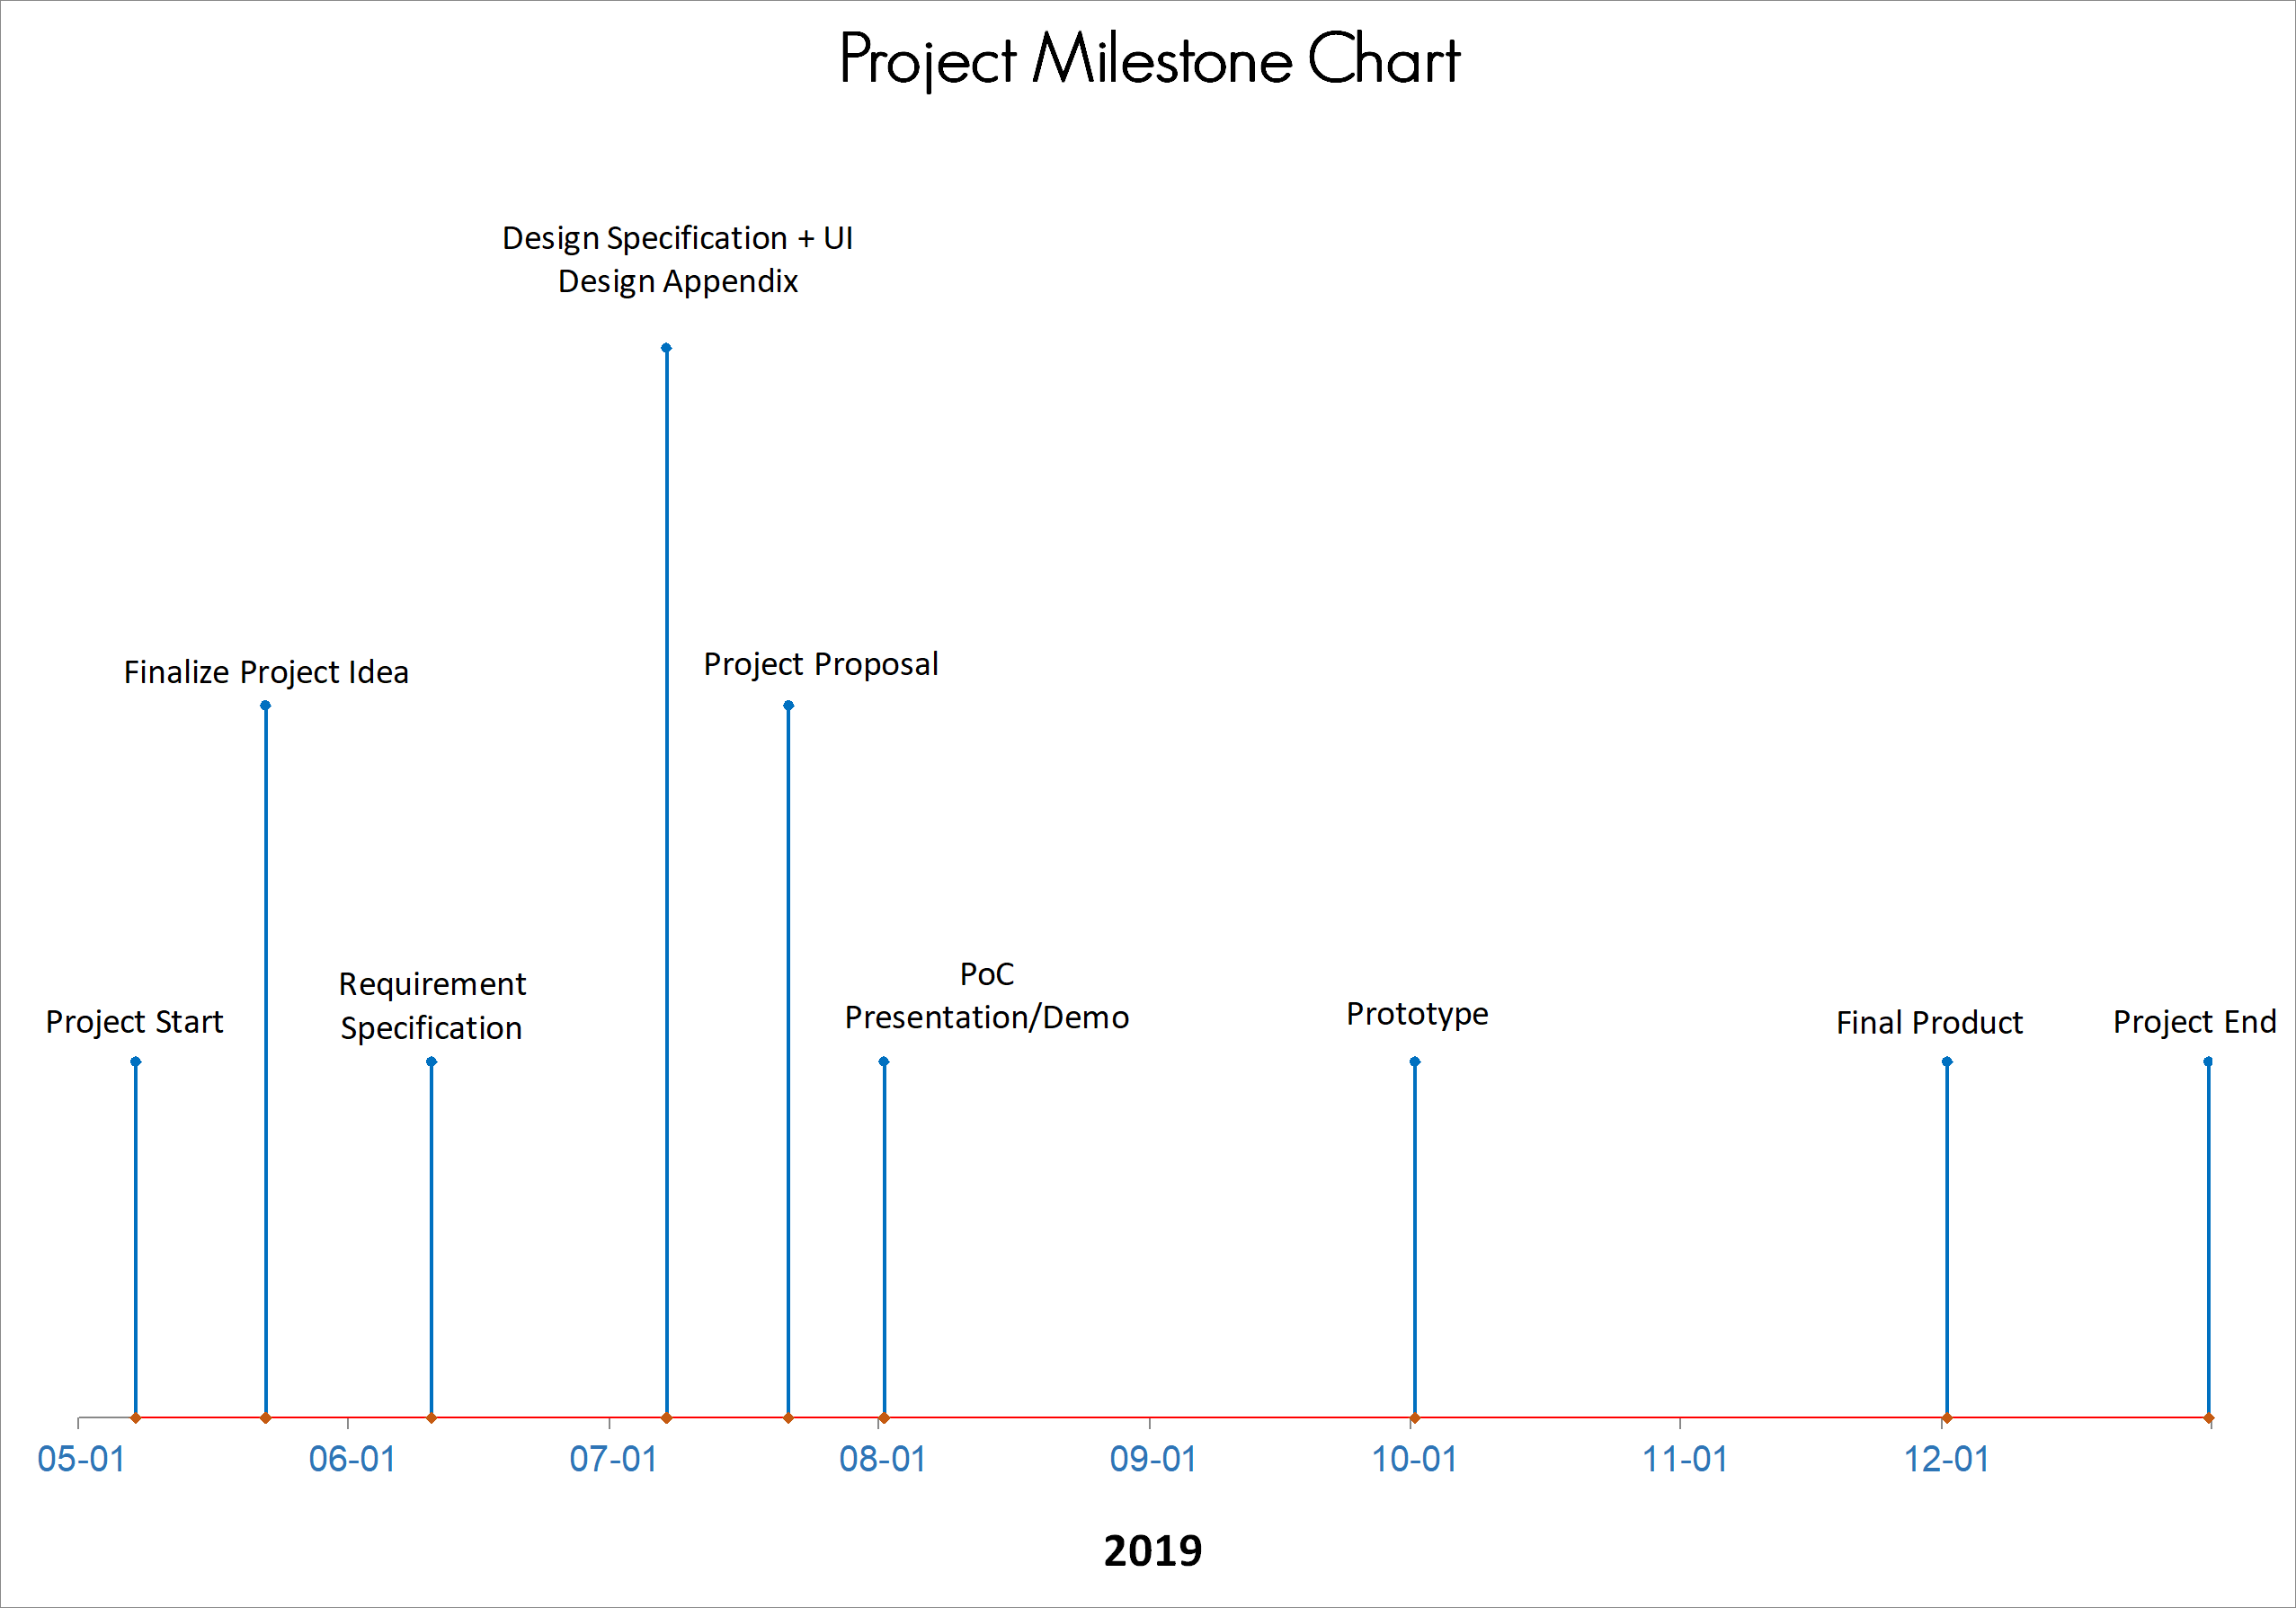
\includegraphics[width=\linewidth]{./images/mile.png}
    \caption{Project Milestone Chart}
    \label{mile}
\end{figure}

\pagebreak
\thispagestyle{empty}
\newgeometry{bottom=2cm,left=2cm,right=2cm,top=2cm}
\begin{landscape}

\begin{figure}
\centering
    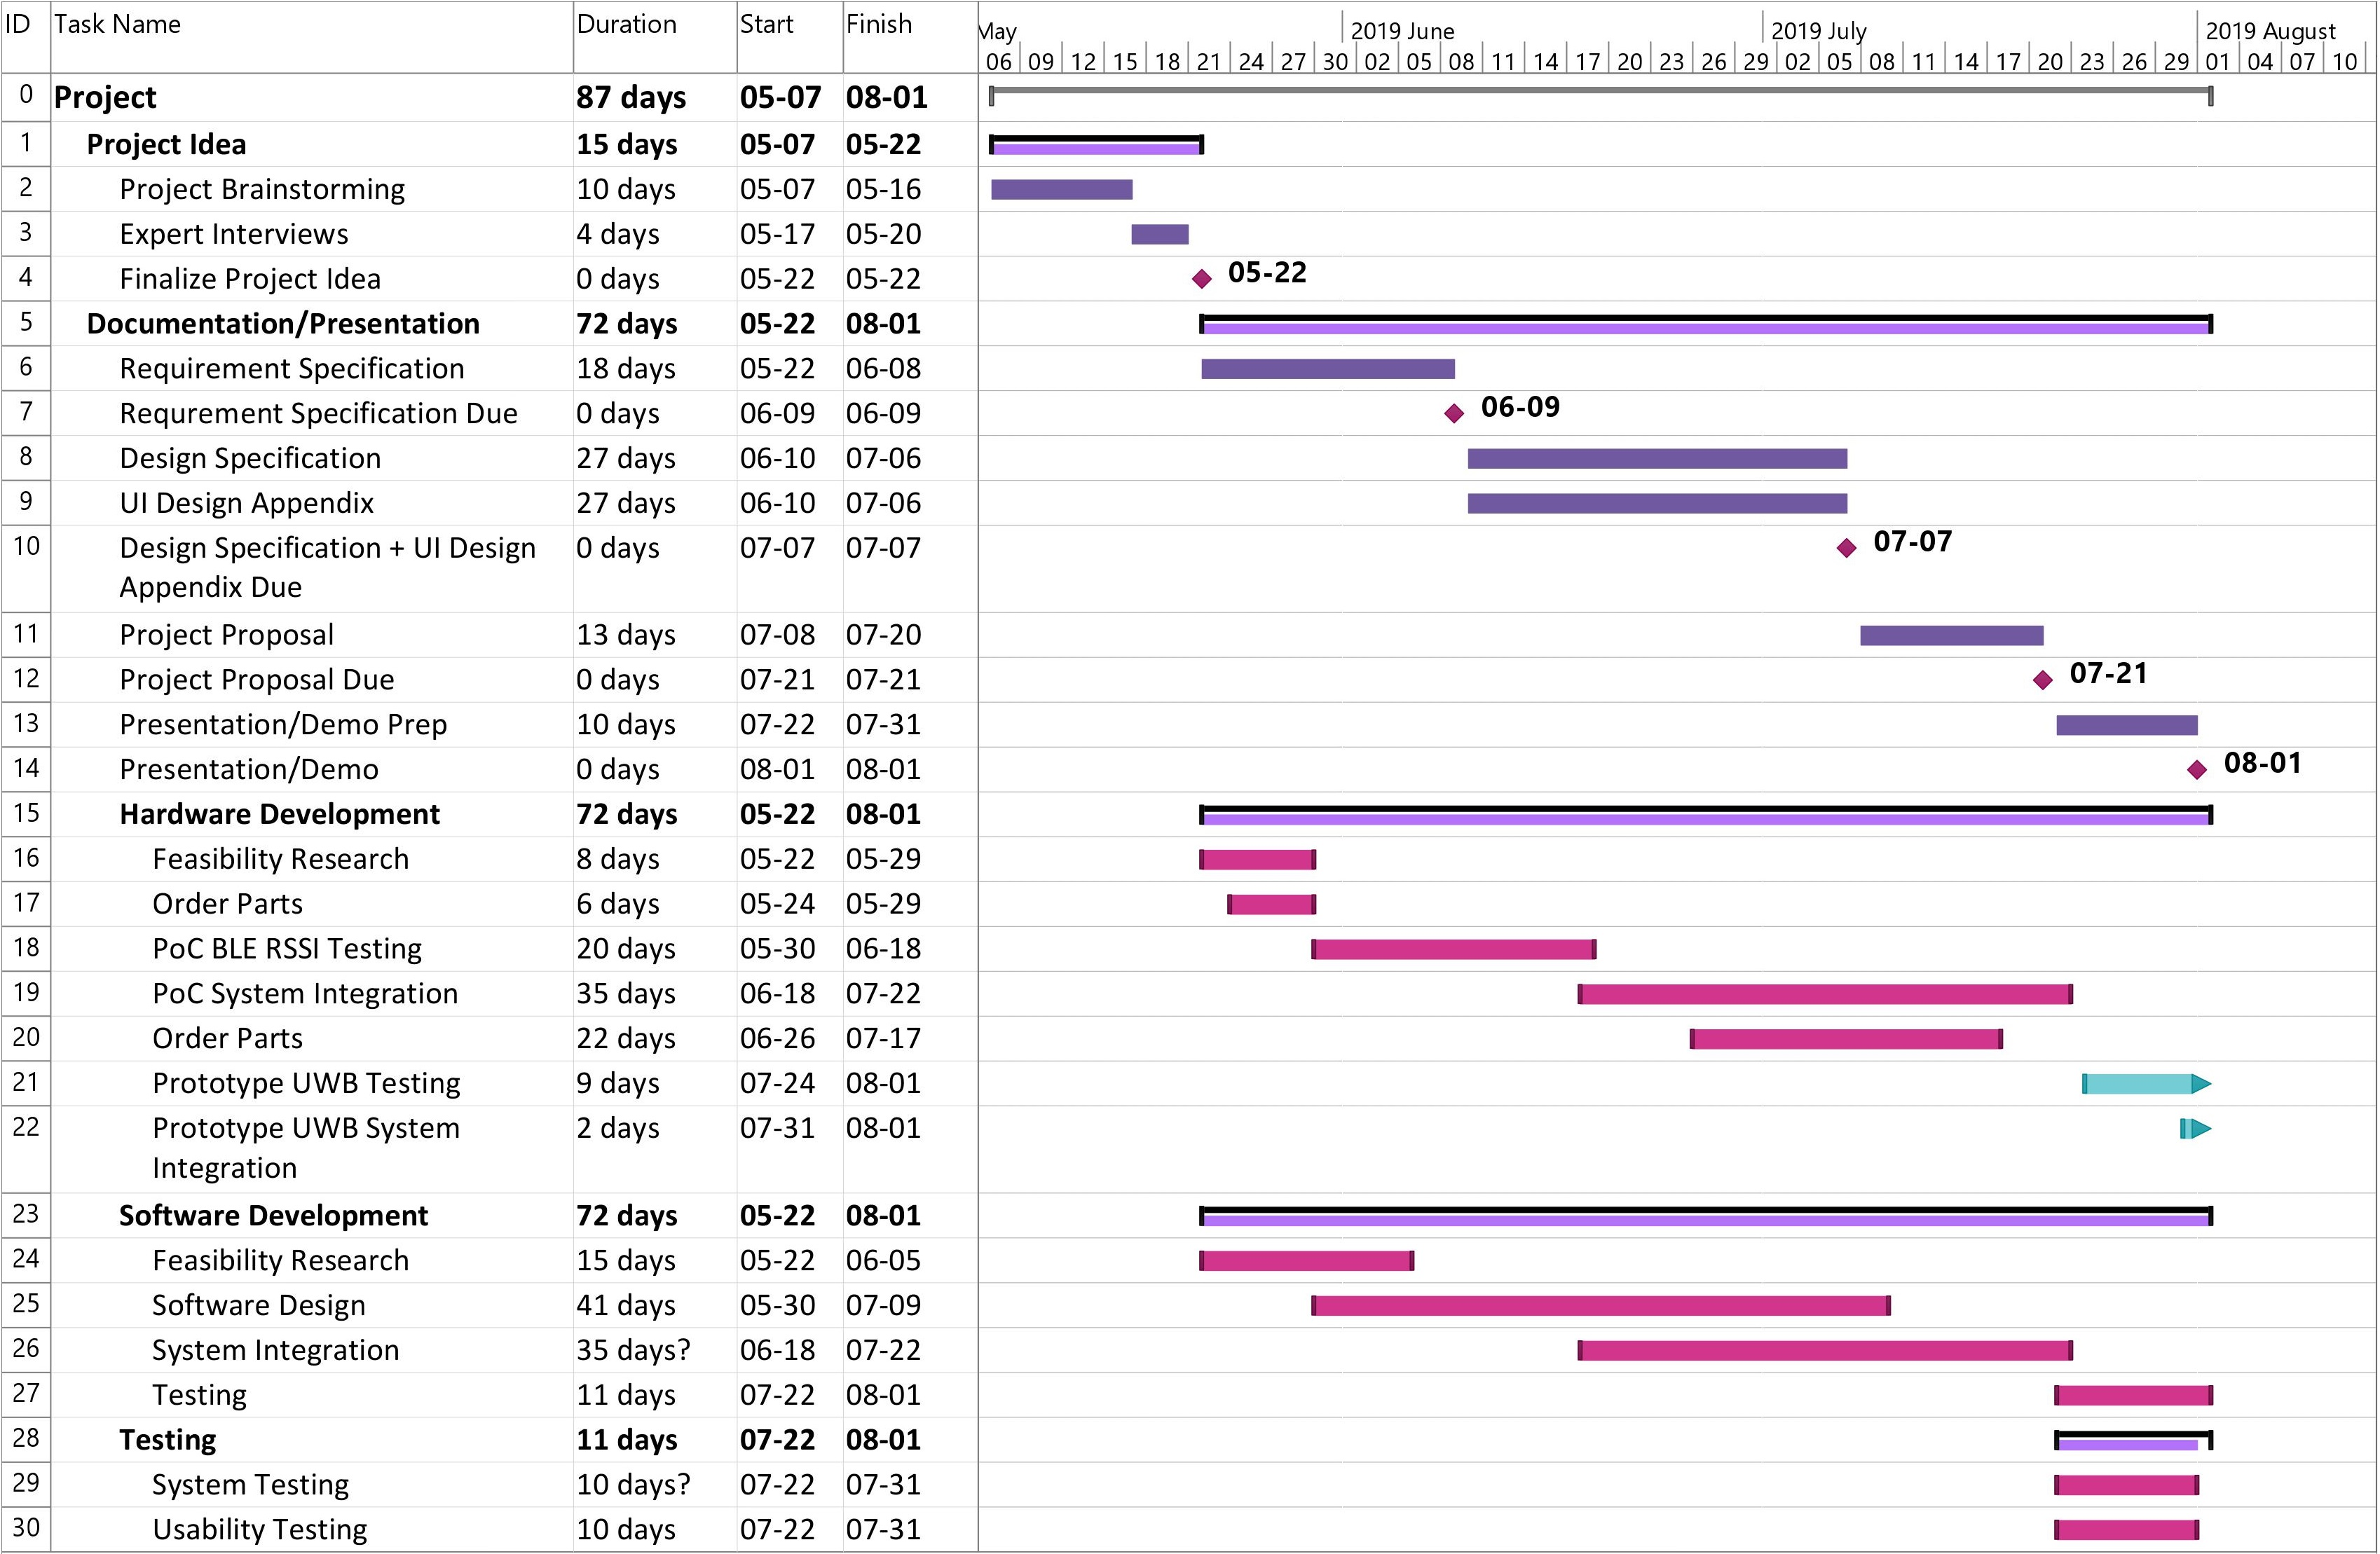
\includegraphics[width=\linewidth]{./images/gantt.jpg}
    \caption{Project Gantt Chart}
    \label{gantt}
\end{figure}
\restoregeometry
\end{landscape}




